\documentclass{seminar}

\usepackage[dvips]{graphicx}
\usepackage{fancybox}
\usepackage{alltt}
\usepackage{amssymb}

\usepackage{labelfig}
\usepackage{url}

% Packages for color.

\usepackage[usenames]{pstcol}
\usepackage{semcolor}
\input{seminar.bug}

\newcommand{\SlideColours}[3]{%
% #1 = frame line color 
% #2 = foreground color
% #3 = background color
% The style frame can be scplain, scshadow, scdouble, none
\slideframe[\psset{linecolor=#1,fillcolor=#3,fillstyle=solid}]{none}%
\color{#2}}
% 

% Basic definitions.

\renewcommand{\printlandscape}{\special{landscape}}    % Works with dvips.
\newcommand{\R}{\mbox{${\mathbb R}$}}
\newcommand{\C}{\mbox{${\mathbb C}$}}
\newcommand{\grad}{\nabla}
\setlength{\jot}{0.0pt}
\newcommand{\half}{{\textstyle{\frac{1}{2}}}}

% Color symbols.

\newcommand{\redball}{\textcolor{BrickRed}{$\bullet$}}
\newcommand{\reddiamond}{\textcolor{BrickRed}{$\diamond$}}
\newcommand{\redcirc}{\textcolor{BrickRed}{$\circ$}}
\newcommand{\redstar}{\textcolor{BrickRed}{$\star$}}
\newcommand{\redplus}{\textcolor{BrickRed}{+}}
\newcommand{\reddash}{\textcolor{BrickRed}{--}}
\newcommand{\redquestion}{\textcolor{BrickRed}{?}}
\newcommand{\redexclaim}{\textcolor{BrickRed}{!}}
\newcommand{\redrightarrow}{\textcolor{BrickRed}{$\Rightarrow$}}

\newcommand{\redstripe}{\textcolor{BrickRed}{\hrule height 2.0pt\hfil}
             \vspace{-1.8pt}
             \textcolor{BrickRed}{\hrule height 1.0pt\hfil}
}

\newcommand{\heading}[1]{%
   \vspace*{0.5pt}%
   \centerline{\textcolor{Blue}{\textbf{#1}}}%
   \redstripe
}

\newcommand{\textblue}[1]{\textcolor{Blue}{\textbf{#1}}}

% Script letters.

\newcommand{\cA} {\mbox{$\cal A$}}
\newcommand{\cB} {\mbox{$\cal B$}}
\newcommand{\cC} {\mbox{$\cal C$}}
\newcommand{\cD} {\mbox{$\cal D$}}
\newcommand{\cF} {\mbox{$\cal F$}}
\newcommand{\cL} {\mbox{$\cal L$}}
\newcommand{\cM} {\mbox{$\cal M$}}
\newcommand{\cP} {\mbox{$\cal P$}}
\newcommand{\cS} {\mbox{$\cal S$}}
\newcommand{\cT} {\mbox{$\cal T$}}

\epsfslidesize

\newpagestyle{MH}
{\hfil Workshop on the ACTS Toolkit  \hfil}
{\hfil \thepage \hfil}

% \pagestyle{MH}
\pagestyle{empty}

\slideframe{Oval}
% \slideframe{none}

%\twoup

\begin{document}

% #1 = frame line color 
% #2 = foreground color
% #3 = background color
% \SlideColours{Black}{Yellow}{NavyBlue}
% \SlideColours{Black}{BlueViolet}{White}

\begin{slide}

\begin{center}
{\bf
Workshop on the ACTS Toolkit \\
September 28--30, 2000 \\
National Energy Research Scientific Computing Center
}
\end{center}

\redstripe

\begin{center}
{\bf
\textcolor{Blue}{TAO -- Toolkit for Advanced Optimization}
}

\redstripe

\medskip

\centerline{\bf Steve Benson, Lois Curfman McInnes, and Jorge J. Mor\'e}

\end{center}

% \medskip

\parbox[b]{3in}{\bf http://www.mcs.anl.gov/tao \bigskip \\
\small  Mathematics and Computer Science Division \\ 
Argonne National Laboratory} 
\includegraphics[scale=0.5]{../images//argonne.ps}

\end{slide}

\begin{slide}

\heading{What is Nonlinearly Constrained Optimization?}

\[
\min \left \{ f(x): x_l \le x \le x_u , \ c_l \le c(x) \le c_u \right \}
\]

\medskip

\begin{list}{\reddiamond}
{
% \setlength{\itemsep}{0pt}
}
\item
Systems of nonlinear equations
\[
\min \left \{ \half \| r(x) \|^2 : x_l \le x \le x_u \right \} , \qquad
r : \R^n \mapsto \R^n
\]
\item
Nonlinear least squares
\[
\min \left \{ \half \| r(x) \|^2 : x_l \le x \le x_u \right \} , \qquad
r : \R^n \mapsto \R^m, \quad m \ge n
\]
\end{list}

\vfill

\end{slide}

\begin{slide}

\heading{What is Nonlinearly Constrained Optimization?}

\[
\min \left \{ f(x): x_l \le x \le x_u , \ c_l \le c(x) \le c_u \right \}
\]

\medskip

\begin{list}{\reddiamond}
{
% \setlength{\itemsep}{0pt}
}
\item
Unconstrained optimization
\[
\min \left \{  f(x) : x \in \R^n \right \}
\]
\item
Bound-constrained optimization
\[
\min \left \{  f(x) : x_l \le x \le x_u \right \}
\]
\item
Linear and quadratic programming
\[
\min \left \{ \half x^T Q x + c^T x : x_l \le x \le x_u , 
\ c_l \le Ax \le c_u \right \}
\]
\end{list}

\vfill

\end{slide}

\begin{slide}

\heading{The Ginzburg-Landau Model for Superconductivity}

Minimize the Gibbs free energy for a homogeneous superconductor with a vector
potential perpendicular to the superconductor.

{\small
\[
\int _ {\cD} \bigl \{ - | v (x) |^2 + \half | v (x) |^4  + 
\left \| \left [ \nabla - i A(x) \right ] v (x) \right \| ^2  +  \\
\kappa^2 \left \| ( \grad \times A ) (x) \right \| ^2 \bigr \} dx
\]
}

\medskip

\begin{center}
$ v : \R^2 \to \C$ is the order parameter

$A : \R^2 \to \R^2 $ is the vector potential
\end{center}

\vfill

\end{slide}

\begin{slide}

\heading{The Ginzburg-Landau Model for Superconductivity}

Unconstrained problem. Non-convex function. Hessian is singular.
Unique minimizer, but there is a saddle point.

\centerline {\includegraphics[height=1.9in]{../images/gl2.eps}}

\end{slide}

\begin{slide}

\heading{Pressure Distribution in a Journal Bearing}

Determine the pressure distribution in a thin film of lubricant
between two circular cylinders

\[
\int_{\cD} \Bigl \{ \half w_q (x) \| \grad v(x) \|^2 - w_l(x) v(x) \Bigr \} \; dx
\]

\[
w_q ( \xi_1 , \xi_2 ) = \left ( 1 + \varepsilon \cos(\xi_1) \right ) ^ 2
\]
\[
w_l ( \xi_1 , \xi_2 ) =  \varepsilon \sin (\xi_1)
\]

\medskip

\begin{center}
$ v \ge 0 $ on the domain $ \cD = ( 0 , 2 \pi ) \times ( 0 , 2 b ) $.
\end{center}

\vfill

\end{slide}

\begin{slide}

\heading{Pressure Distribution in a Journal Bearing}

Bound constrained problem. 
Number of active constraints depends on the eccentricity $ \varepsilon $.
Badly scaled Hessian matrix.
%
\centerline {\includegraphics[height=2.1in]{../images/pjb.eps}}

\end{slide}


\begin{slide}

\heading{Minimal Surface with Obstacles}

Determine the surface of minimal area and given boundary data
that lies above an obstacle.

\[
\min \left \{ f(v) : v \in K \right \}
\]

\[
f(v) = \int_{\cD} \sqrt{ 1 + \| \grad v(x) \|^2 } \; dx
\]

\[
K = \left \{ v \in H^1 : v(x) = v_D (x) , \ x \in \partial D, \ 
                v(x) \ge v_L (x) ,\  x \in \cD \right \}
\]

\vfill

\end{slide}

\begin{slide}

\heading{Minimal Surface with Obstacles}

Bound constrained problem. 
Number of active constraints depends on the height of the
obstacle. All multipliers are zero. 
%
\centerline {\includegraphics[height=2.1in]{../images/mso.eps}}

\end{slide}

\begin{slide}

\heading{Isomerization of $ \alpha $-pinene}

Determine the reaction coefficients
in the thermal isometrization of $\alpha$-pinene from measurements by minimizing
\[
\sum _ {j=1}^8 \| y ( \tau_j ; \theta ) - z_j \| ^ 2 ,
\]
where $z_j$ are the measurements and
\begin{eqnarray*}
y_1'  & = & -(\theta_1 + \theta_2) y_1 \\
y_2'  & = & \theta_1 y_1 \\
y_3'  & = & \theta_2 y_1 - (\theta_3 + \theta_4 )y_3 + \theta_5 y_5 \\
y_4'  & = & \theta_3 y_3 \\
y_5'  & = & \theta_4 y_3 - \theta_5 y_5 \nonumber
\end{eqnarray*}

\end{slide}

\begin{slide}

\heading{Isomerization of $\alpha$-pinene}

Only equality constraints. Typical parameter estimation problem. 

\bigskip

\centerline {\includegraphics[height=1.8in]{../images/pinene.eps}}

\end{slide}

\begin{slide}

\heading{Optimization Toolkits}

State-of-the-art in optimization software:

\begin{list}{\reddiamond}{}
\item
Scattered support for parallel computations
\item
Little reuse of linear algebra software
\item
Minimal use of automatic differentiation software
\item
Few object-oriented optimization codes
\item
Nonlinear optimization problems with more than $ 10, 000 $
variables are considered large.
\end{list}

\vfill

\end{slide}

\begin{slide}

\heading{TAO}

The process of nature by which all things change
and which is to be followed for a life of harmony.

\bigskip

\begin{center}
\textcolor{BrickRed}{The Right Way}
\end{center}

\bigskip

Toolkit for advanced optimization

\begin{list}{\reddiamond}{}
\item
Object-oriented techniques
\item
Component-based interaction
\item
Leverage of existing parallel computing infrastructure
\item
Reuse of external toolkits
\end{list}

\vfill

\end{slide}

\begin{slide}

\heading{TAO Goals}

\begin{list}{\reddiamond}{}
\item
Portability
\item
Performance
\item
Scalable parallelism
\item
An interface independent of architecture
\end{list}

\vfill

\end{slide}


\begin{slide}

\heading{TAO Performance: Journal Bearing Problem (IBM SP)}

\centerline{$ n = 2.56 \cdot 10^6 $ variables}

\small
\begin{table}[htbp]
\begin{center}
\begin{tabular}{| c r | c c r c r |}
\hline
\multicolumn{1}{|c}{$ \varepsilon $} & 
\multicolumn{1}{c|}{$ p $} & 
\multicolumn{1}{c}{faces} &
\multicolumn{1}{c}{$n_{CG}$} & 
\multicolumn{1}{c}{time} &
\multicolumn{1}{c}{$t_{CG}$\%} & 
\multicolumn{1}{c|}{$ \cal E $} \\ \hline
0.1  & 8 & 46 & 431 & 7419 & 86 & 100  \\ 
0.1  & 16 & 45 & 423 & 3706 & 83 & 100  \\
0.1  & 32 & 45 & 427 & 2045 & 82 & 91 \\
0.1  & 64 & 45 & 427 & 1279 & 82 & 73 \\
\hline
0.9  & 8 & 37 & 105 & 2134 & 70 & 100 \\
0.9  & 16 & 37 & 103 & 1124 & 71 & 95 \\
0.9  & 32 & 38 & 100 & 618 & 69 & 86 \\
0.9  & 64 & 38 & 99 & 397 & 68 & 67 \\
\hline
\end{tabular}
\end{center}
\end{table}

\end{slide}


\begin{slide}

\heading{TAO Algorithms (partial list)}

\begin{list}{\reddiamond}
{ \setlength{\itemsep}{0pt}}
\item
Unconstrained optimization 
\begin{list}{\reddash}{}
\item
Conjugate gradient algorithms PR, FR, PR+
\item
Levenberg-Marquardt method (alpha)
\end{list}
\item
Bound-constrained optimization
\begin{list}{\reddash}{}
\item
Limited-memory variable-metric algorithm
\item
Trust region Newton method
% \item
% Gradient projection/conjugate gradient algorithm
\end{list}
\item
Linearly constrained optimization
\begin{list}{\reddash}{}
\item
Interior-point quadratic programming  method (alpha)
\end{list}
\item
Nonlinearly constrained optimization
\begin{list}{\reddash}{}
\item
Work in progress
\end{list}
\end{list}

\end{slide}

\begin{slide}

\heading{TAO Algorithms for Bound-Constrained Optimization}

\[
\min \left \{  f(x) : x_l \le x \le x_u \right \}
\]

\medskip

\begin{list}{\reddiamond}{}
\item
Conjugate gradient algorithms
\item
Limited-memory variable-metric algorithms
\item
Newton algorithms
\end{list}

You must supply the function $ f : \R^n \mapsto \R $ and the
gradient 
\[
\grad f (x) = \left ( \partial _i f(x) \right )
\]

For Newton methods you also need to supply the Hessian matrix.
\[
\grad^2 f (x) = \left ( \partial_{i,j} f(x) \right )
\]

\vfill

\end{slide}

\begin{slide}

\heading{Conjugate Gradient Algorithms}

\[
x_{k+1} = x_k + \alpha_k p_k 
\]
\[
p_{k+1} = - \grad f (x_k) + \beta_k p_k 
\]
where $ \alpha_k $ is determined by a line search.

\medskip

Three choices of $ \beta_k $ are possible ($ g_k = \grad f (x_k ) $):
 
\[
\beta_k^{FR} = \left (
\frac{\| g_{k+1} \|}{\| g_k \|}
\right ) ^ 2 , \qquad \mbox{Fletcher-Reeves}
\]
\[
\beta_k^{PR} = 
\frac{ \langle g_{k+1} , g_{k+1} - g_k \rangle }
{\| g_k \|^2},  \qquad \mbox{Polak-Rivi\`ere}
\]
\[
\beta_k^{PR+} = \max \left \{ \beta_k^{PR} , 0 \right \} , \qquad
\mbox{PR-plus}
\]

\vfill

\end{slide}

\begin{slide}

\heading{Limited-Memory Variable-Metric Algorithms}

\[
x_{k+1} = x_k - \alpha_k H_k \grad f (x_k )
\]
where $ \alpha_k $ is determined by a line search.

\medskip 

The matrix $ H_k $ is defined in terms
of information gathered during the
previous $m$ iterations.

\medskip

\begin{list}{\reddiamond}{}
\item
$ H_k $ is positive definite.
\item
Storage of $ H_k $ requires $ 2 m n $ locations.
\item
Computation of $ H_k \grad f (x_k) $ costs
$ (8m+1) n $ flops.
\end{list}


\vfill

\end{slide}

\begin{slide}

\heading{Trust Region Newton Algorithm}

At each iteration the step $s_k$  (approximately) minimizes 
\[
\min 
\left \{ 
q_k ( x_k + s ) : s_i = 0, \ i \in \cA_k , \
x_l \le x_k + s \le x_u , \ \| s \| \le \Delta_k 
\right \}
\]
where $ q_k $ is the quadratic approximation,
\[
q_k (w) = \langle \grad f (x_k ) , w \rangle + 
\half \langle w , \grad ^2 f(x_k) w \rangle ,
\]
to the function, and $ \Delta_k $ is the trust region bound.
\medskip

\begin{list}{\reddiamond}
{
\setlength{\itemsep}{0pt}
\setlength{\parsep}{0pt}
}
\item
Predict an active set $ \cA_k $.
\item
Compute a step $ s_k $ 
\item
$ x_{k+1} = x_k + s_k $ if $ f (x_k + s_k ) < f (x_k) $, 
otherwise $ x_{k+1} = x_k $.
\item
Update $ \Delta_k $.
\end{list}

\vfill

\end{slide}

\begin{slide}

\heading{TAO Interface}

\begin{alltt}
\scriptsize \setlength{\baselineskip}{10pt}
  TAO_SOLVER tao;                   /* TAO_SOLVER solver context */
  TaoMethod  method=''tao_lmvm''    /* A particular solver method to be used */
  Vec        x, g;                  /* solution and gradient vectors */
  int        n;                     /* number of variables */
  AppCtx     user;                  /* user-defined application context */
  int        info;                  /* status code */

  VecCreate(MPI_COMM_WORLD,n,&x);
  VecDuplicate(x,&g);

  info = TaoCreate(MPI_COMM_WORLD,method,&tao);
  info = TaoSetFunctionGradient(tao,x,g,FunctionGradient,(void *)&user);
  info = TaoSolve(tao);

  info = TaoDestroy(tao);
\end{alltt}

\vfill

\end{slide}

\begin{slide}

\heading{Function Evaluation}

\begin{alltt}
\scriptsize \setlength{\baselineskip}{10pt}
  typedef struct \{         /* Used in the minimum surface area problem */
    int         mx, my;            /* discretization in x, y directions */
    Vec         Bottom, Top, Left, Right;            /* boundary values */
  \} AppCtx;

  int FormFunction(TAO_SOLVER tao, Vec x, double* fcn,void *userCtx)\{
     AppCtx *user = (AppCtx *)userCtx;
     ...
     return 0;
  \}
\end{alltt}
The user sets this routine in the main program via
\begin{alltt}
\scriptsize \setlength{\baselineskip}{10pt}
    info = TaoSetFunction(tao,x,FormFunction,(void *)&user);
\end{alltt}

\vfill

\end{slide}

\begin{slide}

\heading{Gradient Evaluation}

\begin{alltt}
\scriptsize \setlength{\baselineskip}{10pt}
  int FormGradient(TAO_SOLVER tao, Vec x, Vec g,void *userCtx)\{
     AppCtx *user = (AppCtx *)userCtx;
     ...
     return 0;
\}
\end{alltt}

The user sets this routine in the main program via
\begin{alltt}
\scriptsize \setlength{\baselineskip}{10pt}
    info = TaoSetGradient(tao,g,FormGradient,(void *)&user);
\end{alltt}
Alternatively, the user can supply the function and gradient evaluation
in a single routine.

\medskip

A Hessian evaluation routine can be supplied in a similar manner.

\vfill

\end{slide}

\begin{slide}

\heading{Convergence}

Absolute tolerances specify acceptable errors in the optimality of the function
and the constraints.
\[ f(x) \leq f(x^*) + \epsilon_{fatol} \]
Relative tolerances specify the number of significant digits required
in the solution and the constraints.
\[ 
f(x) \leq f(x^*) + \epsilon_{frtol} | f(x^*) |
\]

These tolerance can be changed
\begin{alltt}
\scriptsize \setlength{\baselineskip}{10pt}
    int TaoSetTolerances(TAO_SOLVER solver,double fatol,double frtol,
                                           double catol,double crtol)
\end{alltt}

\vfill

\end{slide}

\begin{slide}

\heading{TAO Basic Facilities}

\begin{list}{\reddiamond}{}
\item
TaoSetInitialVector
\item
TaoSetBounds
\item
TaoGetSLES
\item 
TaoGetFunctionValue
\item
TaoCheckSuccess
\item
TaoView
\end{list}

\vfill

\end{slide}

\begin{slide}

\heading{Parallel Functionality}

The TAO interface is the same in a parallel environment, but the user
must provide vectors with a parallel structure.
\begin{alltt}
\scriptsize \setlength{\baselineskip}{10pt}
  VecCreateMPI(MPI_COMM_WORLD,n,PETSC_DECIDE,&x);
  VecDuplicate(x,&g);

  info = TaoCreate(MPI_COMM_WORLD,method,&tao);
  info = TaoSetFunctionGradient(tao,x,g,FunctionGradient,(void *)&user);
  info = TaoSolve(tao);

  info = TaoDestroy(tao);
\end{alltt}
The user still provides the routines that evaluate the function and
gradient.  These routines do not have to be performed in parallel,
but parallel evaluations usually improve performance.
\end{slide}


\begin{slide}

\heading{Parallel Function Evaluation}

\begin{alltt}
\scriptsize \setlength{\baselineskip}{10pt}
   typedef struct \{                    /* For Minimum Surface Area Problem */
     int         mx, my;              /* discretization in x, y directions */
     Vec         Bottom, Top, Left, Right;              /* boundary values */
     Vec         localX, localG;                   /* ghosted local vector */
     DA          da;                   /* distributed array data structure */
   \} AppCtx;

   int FormFunction(TAO_SOLVER tao, Vec x, double* fcn,void *userCtx)\{
      AppCtx *user = (AppCtx *)userCtx;
      ...
      info = MPI_Allreduce(&f,fcn,1,MPI_DOUBLE,MPI_SUM,MPI_COMM_WORLD);
      return 0;
   \}
\end{alltt}

\vfill

\end{slide}

\begin{slide}
\heading{Where Can We Find TAO?}

At {\bf http://www.mcs.anl.gov/tao}

\begin{list}{\reddiamond}{\leftmargin=1in}
\item
Source Code
\item
Documentation
\item
Installation Instructions
\item
Example Problems
\item
Additional Tutorials
\item
Performance Results
\item
Supported Architectures
\end{list}

\vfill

\end{slide}


\end{document}


